\section{Основная часть}
    Перед началом создания обработки нужно разобраться в структуре бизнес-процесса замены картриджей.

    \subsection{Структура бизнес-процесса}
    Бизнес-процесс в системе 1С -- это последовательности определённых задач, выполняемых разными сотрудниками. Когда очередной пользователь выполнит свою задачу, программа создаст задачу для следующего.

    Каждая задача имеет своего исполнителя и, в зависимости от результата выполнения, запускает за собой определённую задачу из бизнес-процесса. Последовательность задач бизнес-процесса представлена в виде карты справа снизу на интерфейсе бизнес-процесса (Рис. \ref{process}).

    \begin{figure}[H]
        \centering
        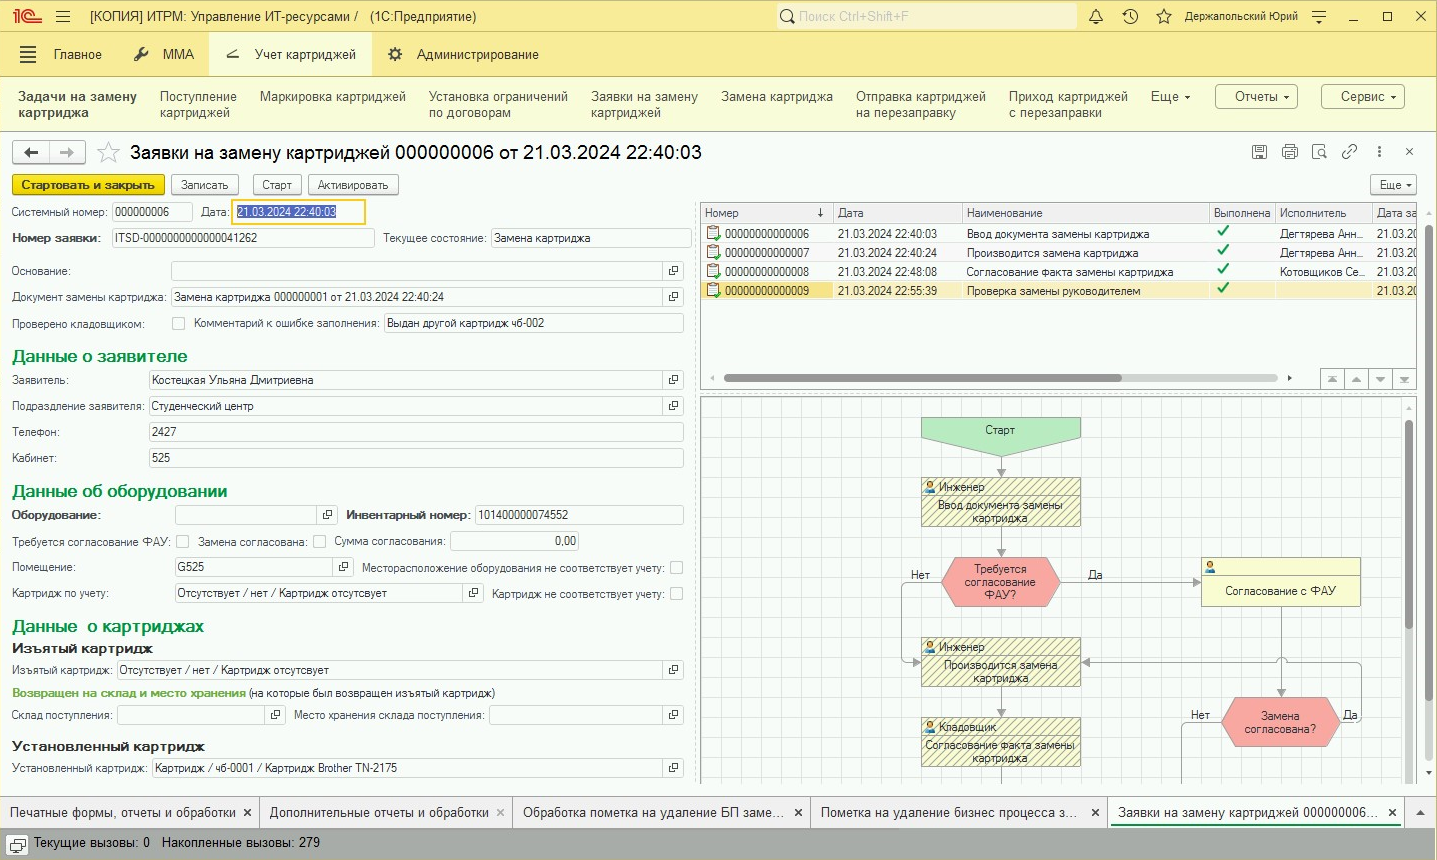
\includegraphics[width=14cm]{pictures/process.png}
        \caption{Интерфейс бизнес-процесса замены картриджей.}  \label{process}
    \end{figure}

    Также, если завершена первая задача процесса <<Ввод документа замены картриджа>>, то в системе появляется документ замены картриджа, который соответствует данному процессу.

    Далее наименование и действие задачи не будет иметь значения, поскольку в системе они все имеют тип <<Задача>>.

    В итоге имеем объекты, которые необходимо пометить на удаление: бизнес-процесс, задачи бизнес-процесса и документ замены.

    \subsection{Программное определение необходимых объектов и создание формы}
    Для начала, пользователь, который будет использовать обработку, должен выбрать бизнес процесс. Для этого используется базовый функционал формы 1С. Создаётся реквизит (в 1С так называется параметр) формы/обработки, который имеет базовый функционал выбора из списка существующих бизнес-процессов. 

    У бизнес-процесса есть ссылка на соответствующий документ замены. Если документа ещё нет, то ссылка будет пустой, поэтому её везде нужно проверять на то, пустая ли она. При выборе бизнес-процесса будет заполняться реквизит документа замены по ссылке на него.
    
    Бизнес-процесс не имеет ссылок на задачи, однако все задачи имеют ссылку на бизнес-процесс. Поэтому для поиска соответствующих задач будет использоваться запрос. Запросы в 1С являются аналогами запросов SQL. Из таблицы всех задач выбираются те, у которых ссылка на бизнес-процесс совпадает с введённым бизнес-процессом. У каждой задачи выбирается ссылка, а также для визуализации: номер, дата, наименование, выполнение задачи (Рис. \ref{query1}).
    
    \begin{figure}[H]
        \centering
        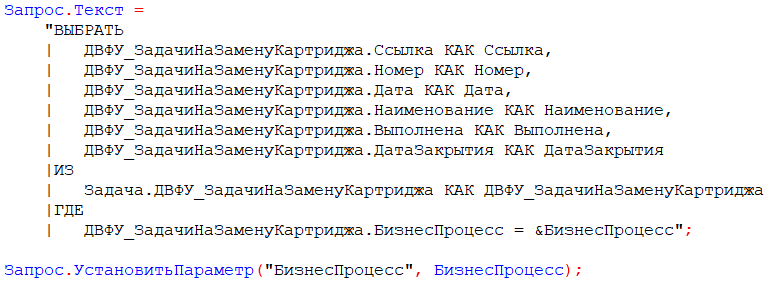
\includegraphics[width=10cm]{pictures/query1.png}
        \caption{Запрос для выбора задач по бизнес-процессу.}  \label{query1}
    \end{figure}
    
    Полученные задачи заполняют таблицу значений. На форме бизнес-процесса имеется возможность открыть задачу из списка, поэтому на форме обработки нужно сохранить соответствующий функционал: открывать нужную форму со ссылкой задачи (Рис. \ref{clicked}), однако убрать возможность редактирования, установив параметр <<ТолькоПросмотр>>.

    Для того, чтобы помечать полученные объекты на удаление нужно создать команду, которая будет выполняться при нажатии на кнопку. Для этого нужно будет вызывать функцию, которая будет работать в контексте сервера (в 1С такие функции и процедуры могут, например, получать все свойства объектов по ссылкам) для того, чтобы получить объект по ссылке и пометить его на удаление. Также для удобства пользователя была добавлена кнопка, которая уберёт пометку на удаление со всех объектов.

    После того, как произойдёт пометка нужно сообщить пользователю о пометке. Для этого текст в полях бизнес-процесса и документа замены будут покрашены в красный цвет, если помечены на удаление. Если пометка, наоборот, убиралась, то текст будет покрашен обратно в чёрный. В таблице задач будет показываться иконка с красным крестом, если задача помечена на удаление, а иконка задачи иначе.
    
    Вся форма и пример с помеченными объектами показана на рисунке \ref{form}.

    Ещё одним состоянием бизнес-процесса является закрыт ли он или нет. Если процесс закрыт, то его нельзя будет пометить на удаление, а кнопки команд пометки будут выключены.

    \begin{figure}[H]
        \centering
        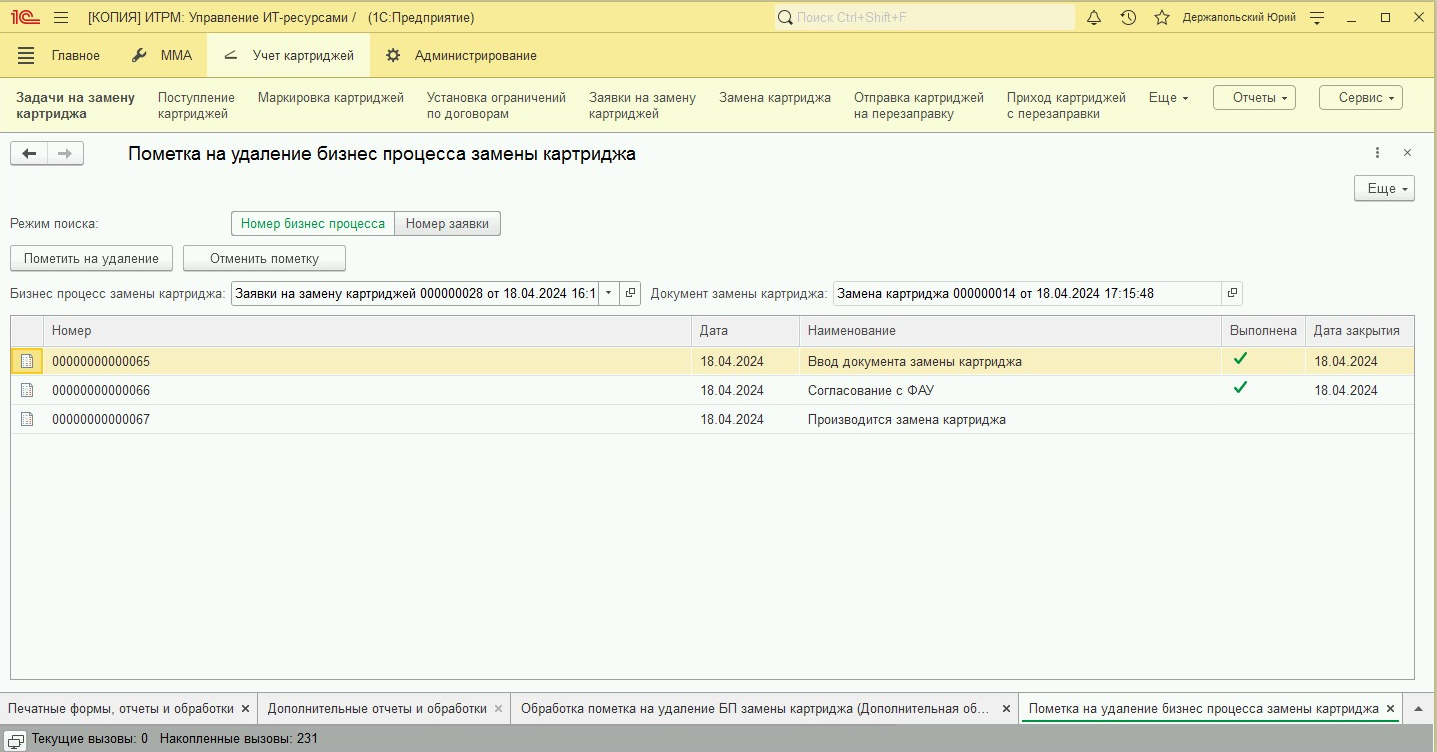
\includegraphics[width=13cm]{pictures/interf.png}
        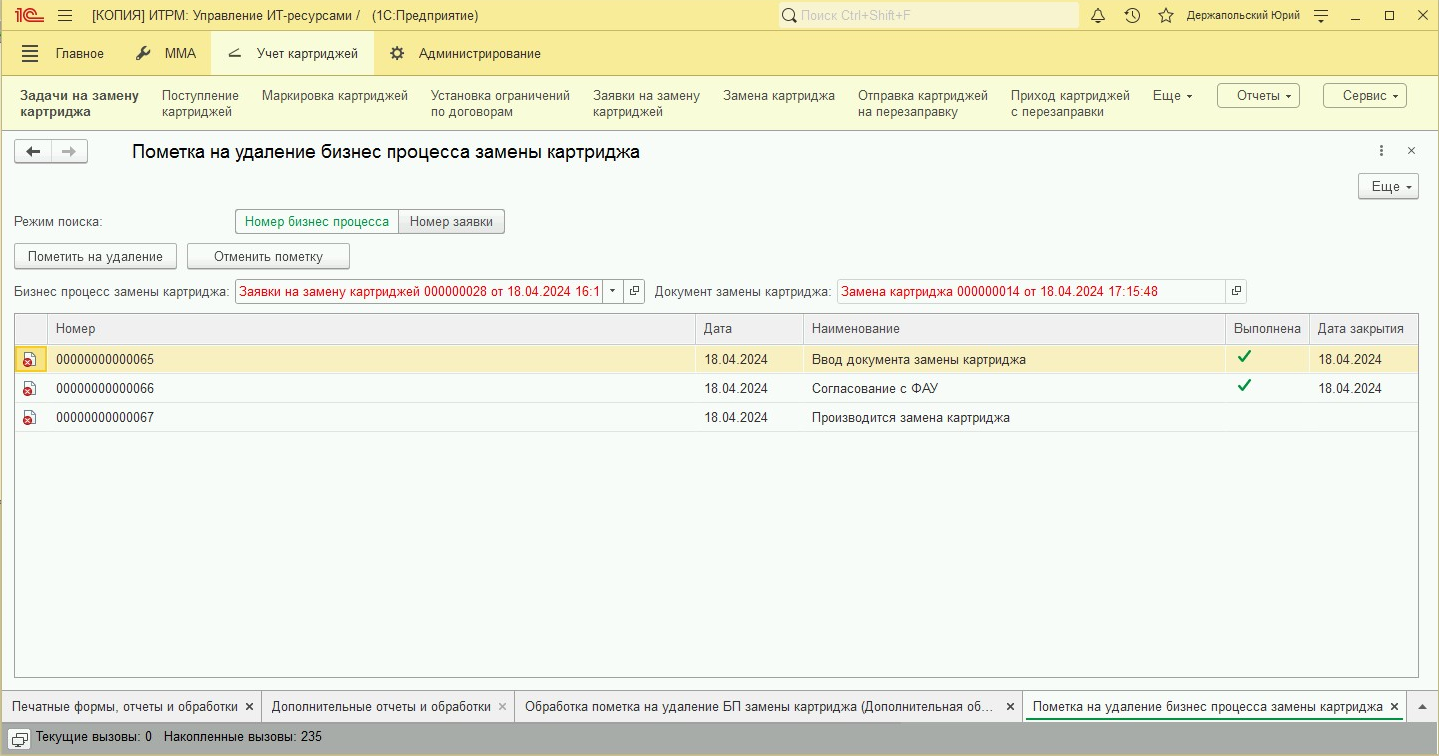
\includegraphics[width=13cm]{pictures/interf_marked.png}
        \caption{Форма внешней обработки без метки на удаление и с меткой.}  \label{form}
    \end{figure}

    \subsection{Разделение способов нахождения бизнес-процесса}
    Описанная выше форма используется для выбора конкретного бизнес-процесса. Однако, описанная проблема во введении решена не до конца. Если процессы имеют одинаковый номер заявки (дубликаты и т.д.), то при выборе из списка эти номера не показываются. Для решения этого нужно добавить другой режим поиска -- по номеру заявки.

    На форме нужно добавить строку поиска для номера. При нажатии на кнопку поиска будет выполняться запрос (Рис. \ref{query2}), который из таблицы бизнес-процессов будет выбирать их с условием на подобность введённой строки (т.е. поиск подстроки в номере процесса).
    
    \begin{figure}[H]
        \centering
        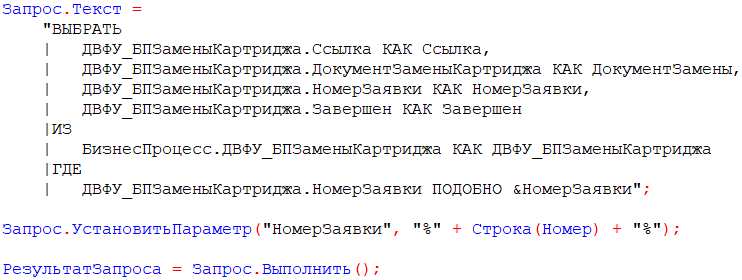
\includegraphics[width=10cm]{pictures/query2.png}
        \caption{Запрос для выбора бизнес-процессов по подобию номеру.}  \label{query2}
    \end{figure}
    
    Полученные процессы будут заполнять соответствующую таблицу значений. 

    При нажатии на бизнес-процесс в таблице он будет заполнять реквизит бизнес-процесса на форме, описанный в предыдущем пункте, аналогично заполняя таблицу задач и реквизит документа замены.

    При нажатии на кнопку пометки работает та же функция, а также в таблице бизнес-процессов меняется иконка.

    Для переключения режимов вверху формы есть тумблер. При переключении появляются и скрываются только таблица бизнес-процессов и строка поиска номера. Также в строке выбора бизнес-процесса включается и отключается возможность выбора. При переключении также стираются все данные поиска.

    На рисунке \ref{list} показана форма режима поиска по номеру.

    \begin{figure}[H]
        \centering
        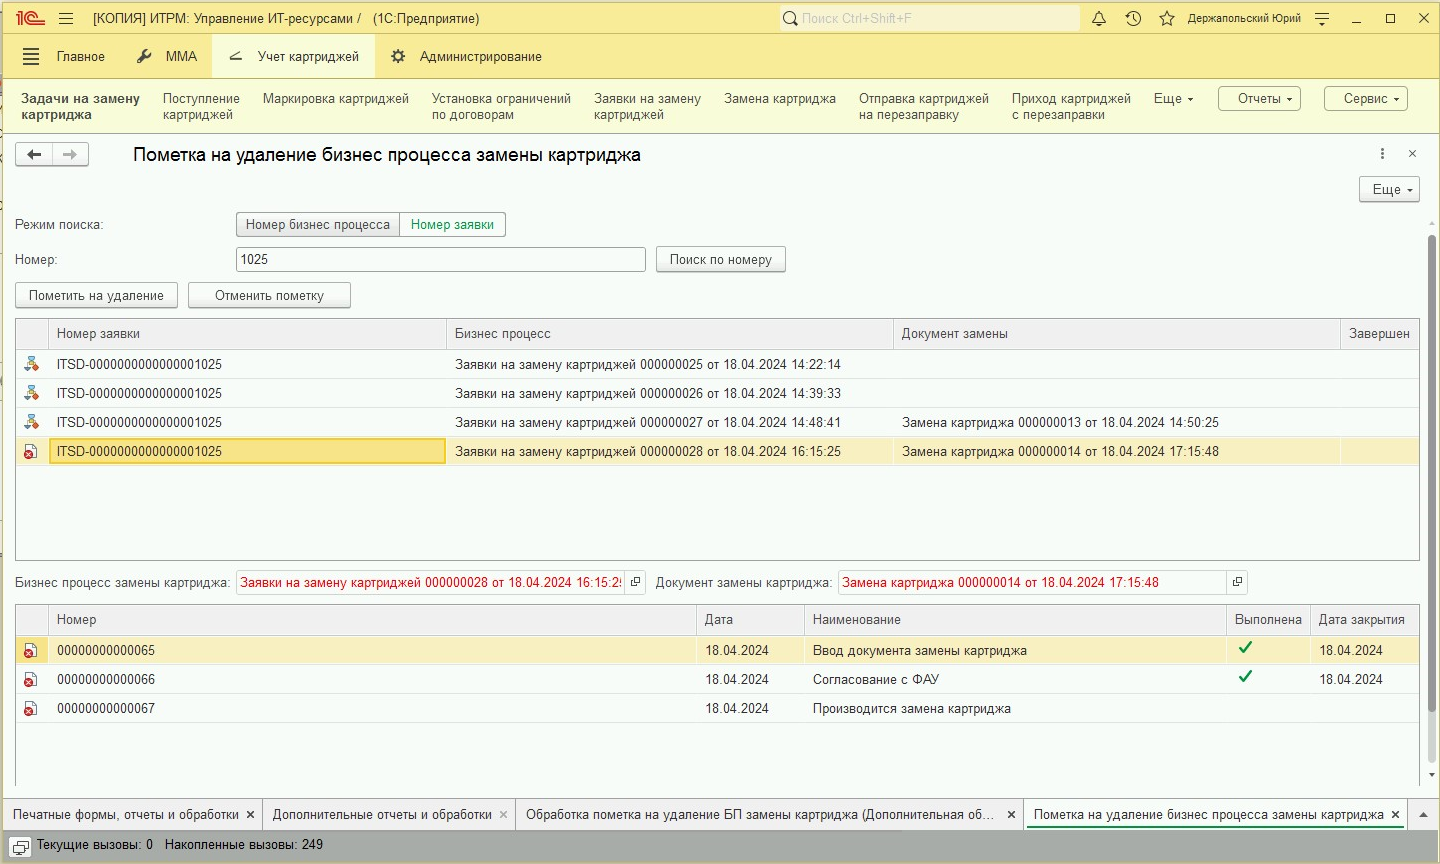
\includegraphics[width=12cm]{pictures/interf_list.png}
        \caption{Режим поиска по номеру.}  \label{list}
    \end{figure}

    \begin{figure}[H]
        \centering
        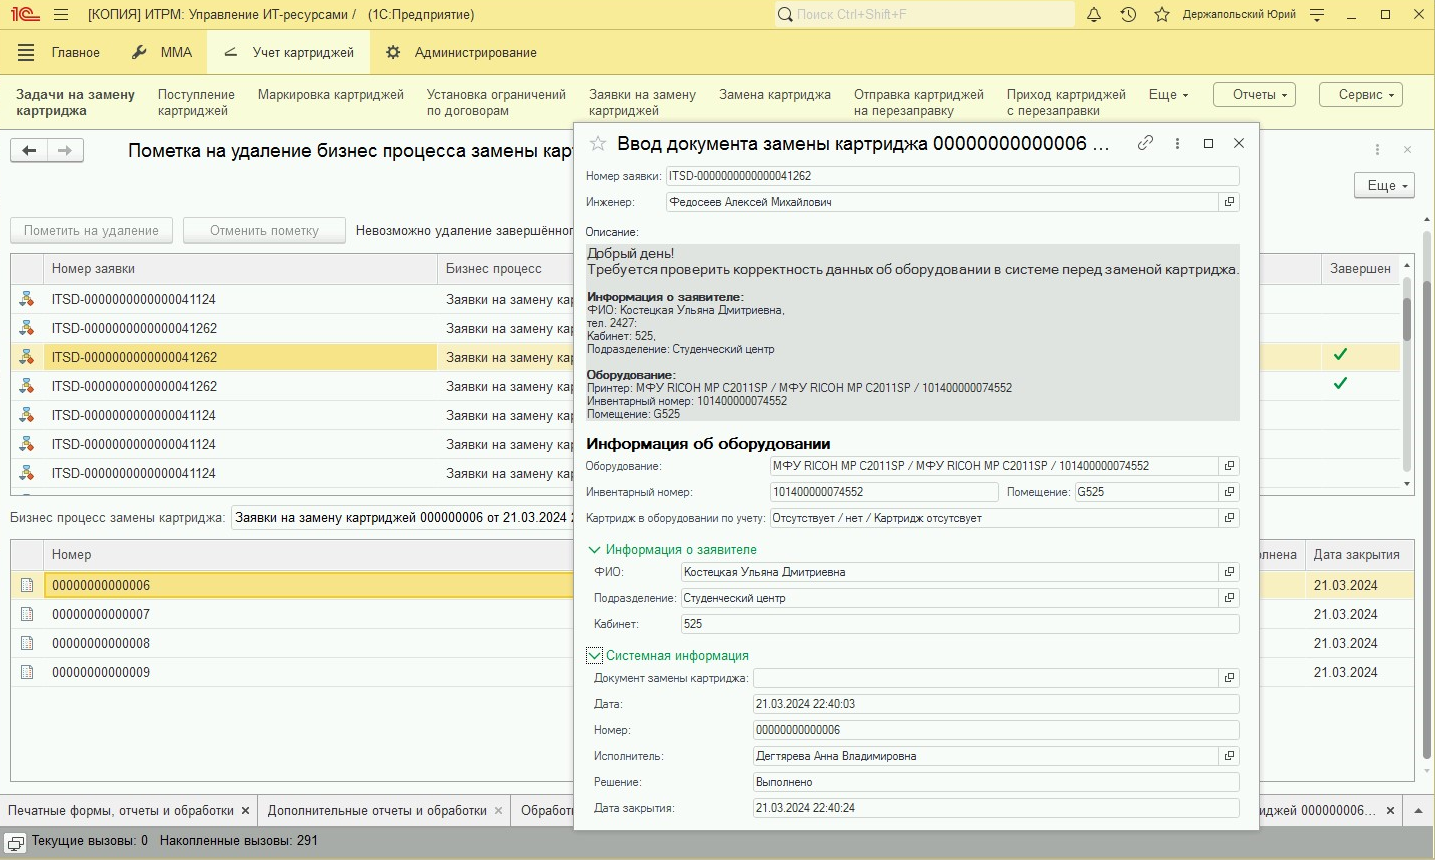
\includegraphics[width=12cm]{pictures/clicked.png}
        \caption{Открытая задача через таблицу задач.}  \label{clicked}
    \end{figure}

    \subsection{Интеграция в систему 1С}
    Для того, чтобы использовать внешнюю обработку непосредственно в системе 1С нужно её <<зарегистрировать>>, т.е. в самой обработке написать дополнительную информацию, нужную для распознавания системой 1С. Для этого используются функции БСП (библиотека стандартных подсистем). На рисунке \ref{external} показана загруженная в систему обработка. 

    \begin{figure}[H]
        \centering
        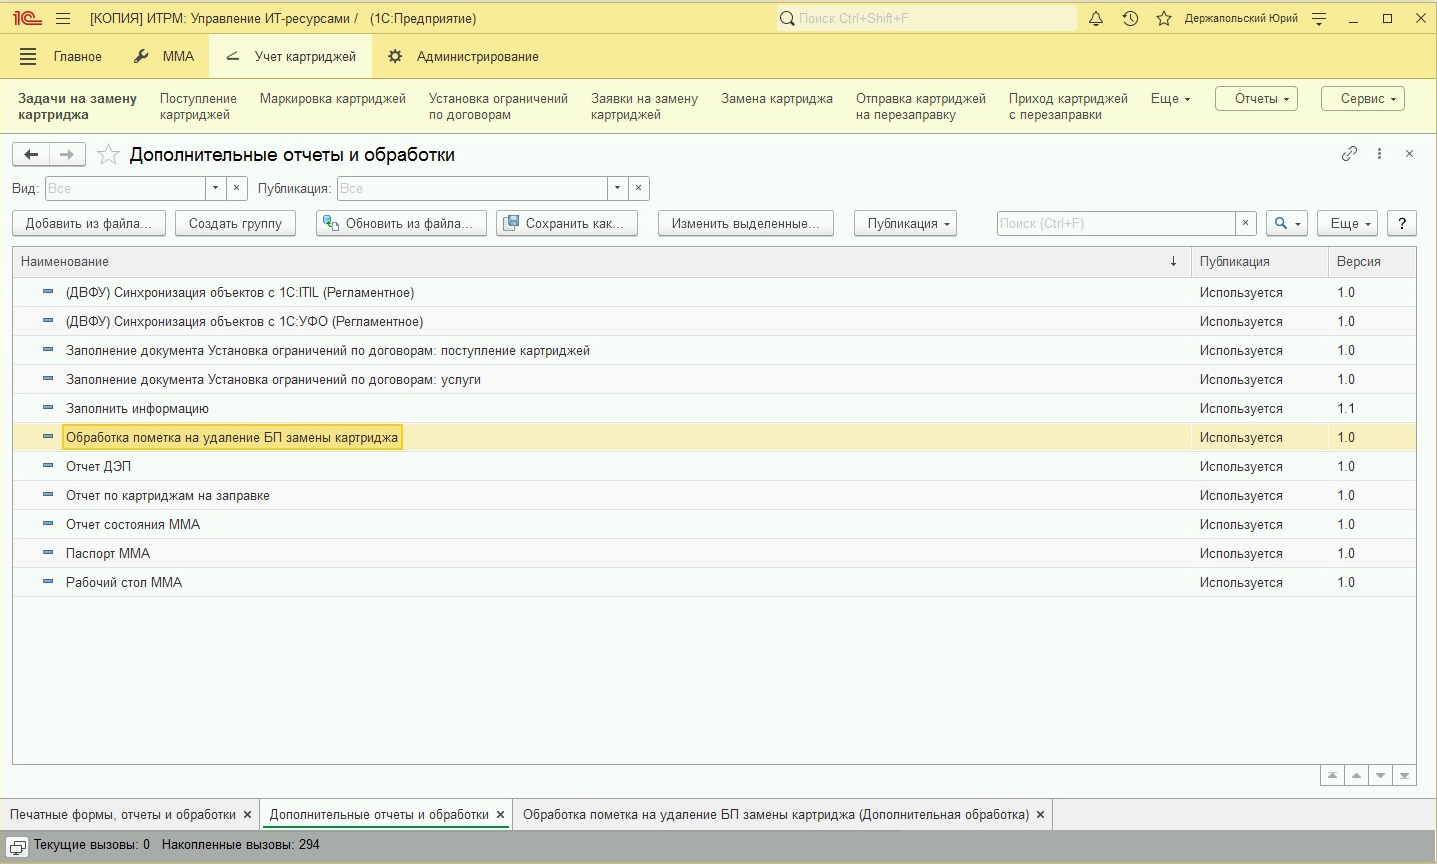
\includegraphics[width=12cm]{pictures/external.png}
        \caption{Обработка среди других дополнительных отчётов и обработок.}  \label{external}
    \end{figure}